%\documentclass[12pt]{article}  % standard LaTeX, 12 point type
\documentclass[sigconf]{acmart}

\usepackage{booktabs} % For formal tables
\usepackage{multirow}
\usepackage{listings}   

\usepackage{amsfonts,latexsym}
\usepackage{amsthm}
\usepackage{amssymb}
\usepackage[utf8x]{inputenc} % Кодировка
\usepackage[english]{babel} % Многоязычность
\usepackage{amsmath}
\usepackage{tikz}
\usetikzlibrary{automata,positioning}
\usetikzlibrary{graphs, graphs.standard, quotes}
\usetikzlibrary{arrows,decorations.pathmorphing,backgrounds,positioning,fit,petri}


\usepackage{algpseudocode}
\usepackage{algorithm}
\usepackage{caption}
\usepackage{algorithmicx}
\usepackage{systeme}



\newtheorem{theorem}{Theorem}[section]
\newtheorem{proposition}[theorem]{Proposition}
\newtheorem{lemma}[theorem]{Lemma}
\newtheorem{corollary}[theorem]{Corollary}
\newtheorem{conjecture}[theorem]{Conjecture}

\theoremstyle{definition}
\newtheorem{definition}{Определение}[section]
\newtheorem{example}{Example}[section]

% unnumbered environments:

\theoremstyle{remark}
\newtheorem*{remark}{Remark}
\newtheorem*{notation}{Notation}
\newtheorem*{note}{Note}

\setlength{\parskip}{5pt plus 2pt minus 1pt}
%\setlength{\parindent}{0pt}

\usepackage{color}
\usepackage{listings}
\usepackage{caption}
\usepackage{graphicx}
\usepackage{ucs}

\setcounter{MaxMatrixCols}{20}


\newcommand{\tab}[1][0.3cm]{\ensuremath{\hspace*{#1}}}
% A generalized view on parsing and translation
% http://dl.acm.org/citation.cfm?id=2206331
\title{Rytter-style Algorithm for Context-Fre Path Querying}

\author{Semyon Grigorev}
\orcid{0000-0002-7966-0698}
\affiliation{%
  \institution{Saint Petersburg State University}
  \streetaddress{7/9 Universitetskaya nab.}
  \city{St. Petersburg}
  \country{Russia}
  \postcode{199034}
}
\email{semen.grigorev@jetbrains.com}


\author{Ekaterina Shemetova}
\affiliation{%
  \institution{Saint Petersburg State University}
  \streetaddress{7/9 Universitetskaya nab.}
  \city{St. Petersburg}
  \country{Russia}
  \postcode{199034}
}
\email{katyacyfra@gmail.com}




\date{\today}

\textwidth=190mm
\textheight=250mm
\topmargin=-20mm
\oddsidemargin=-15mm
\evensidemargin=-15mm


\begin{document}

\algtext*{EndWhile}% Remove "end while" text
\algtext*{EndIf}% Remove "end if" text
\algtext*{EndFor}% Remove "end for" text
\algtext*{EndFunction}% Remove "end function" text


%\begin{abstract}
%Abstract
%\end{abstract}

%
% The code below should be generated by the tool at
% http://dl.acm.org/ccs.cfm
% Please copy and paste the code instead of the example below.
%
%\begin{CCSXML}
%<ccs2012>
%<concept>
%<concept_id>10002951.10002952.10002953.10010146</concept_id>
%<concept_desc>Information systems~Graph-based database models</concept_desc>
%<concept_significance>500</concept_significance>
%</concept>
%<concept>
%<concept_id>10002951.10002952.10003197.10010825</concept_id>
%<concept_desc>Information systems~Query languages for non-relational engines</concept_desc>
%<concept_significance>500</concept_significance>
%</concept>
%<concept>
%<concept_id>10011007.10011006.10011008.10011009.10011012</concept_id>
%<concept_desc>Software and its engineering~Functional languages</concept_desc>
%<concept_significance>300</concept_significance>
%</concept>
%<concept>
%<concept_id>10003752.10003766.10003771</concept_id>
%<concept_desc>Theory of computation~Grammars and context-free languages</concept_desc>
%<concept_significance>300</concept_significance>
%</concept>
%</ccs2012>
%\end{CCSXML}

%\ccsdesc[500]{Information systems~Graph-based database models}
%\ccsdesc[500]{Information systems~Query languages for non-relational engines}
%\ccsdesc[300]{Software and its engineering~Functional languages}
%\ccsdesc[300]{Theory of computation~Grammars and context-free languages}

%\keywords{Graph Databases, Language-Constrained Path Problem, Context-Free Path Querying, Parser Combinators, Generalized LL, GLL, Neo4J, Scala}


\maketitle

%\section{Introduction}


Language-constrained path querying~\cite{barrett2000formal} is a technique for graph navigation querying.
This technique allows one to use formal languages as constraints on paths in edge-labeled graphs: path satisfies constraints if labels along it form a word from the specified language.

The utilization of regular languages as constraints, or \textit{Regular Path Querying} (RPQ), is most well-studied and widespread.
Different aspects of RPQs are actively studied in graph databases~\cite{10.1145/2463664.2465216, 10.1145/3104031,10.1145/2850413}, while regular constraints are supported in such popular query languages as PGQL~\cite{10.1145/2960414.2960421} and SPARQL\footnote{Specification of regular constraints in SPARQL property paths: \url{https://www.w3.org/TR/sparql11-property-paths/}. Access date: 07.07.2020.}~\cite{10.1007/978-3-319-25007-6_1} (property paths).
Nevertheless, there is certainly room for improvement of RPQ efficiency, and new solutions are being created~\cite{Wang2019,10.1145/2949689.2949711}.

At the same time, using more powerful languages, namely context-free languages, as constraints has gained popularity in the last few years.
\textit{Context-Free Path Querying} problem (CFPQ) was introduced by Mihalis Yannakakis in 1990 in~\cite{Yannakakis}.
Many algorithms were proposed since that time, but recently, Jochem Kuijpers et al. showed in~\cite{Kuijpers:2019:ESC:3335783.3335791} that state-of-the-art CFPQ algorithms are not performant enough for practical use.
This motivates us to develop new algorithms for CFPQ.

One promising way to achieve high-performance solutions for graph analysis problems is to reduce them to linear algebra operations.
This way, GraphBLAS~\cite{7761646} API, the description of basic linear algebra primitives, was proposed.
Solutions that use libraries that implement this API, such as SuiteSparce~\cite{10.1145/3322125} and CombBLAS~\cite{10.1177/1094342011403516}, show that reduction to linear algebra is a way to utilize high-performance parallel and distributed computations for graph analysis.

Rustam Azimov shows in~\cite{Azimov:2018:CPQ:3210259.3210264} how to reduce CFPQ to matrix multiplication.
Later, it was shown in~\cite{Mishin:2019:ECP:3327964.3328503} and~\cite{10.1145/3398682.3399163} that utilization of appropriate libraries for linear algebra for Azimov's algorithm implementation makes a practical solution for CFPQ.
However Azimov's algorithm requires transforming the input grammar to Chomsky Normal Form, which leads to the grammar size increase, and hence worsens performance, especially for regular queries and complex context-free queries.

To solve these problems, an algorithm based on automata intersection was proposed~\cite{10.1007/978-3-030-54832-2_6}.
This algorithm is based on linear algebra and does not require the transformation of the input grammar.
We improve the algorithm in this work.
We reduce the above mentioned solution to operations over Boolean matrices, thus simplifying its description and implementation.
Also, we show that this algorithm is performant enough for regular queries, so it is a good candidate for integration with real-world query languages: one algorithm can be used to evaluate both regular and context-free queries.

Moreover, we show that this algorithm opens the way to tackle a long-standing problem about the existence of truly-subcubic $O(n^{3-\epsilon})$ CFPQ algorithm ~\cite{10.1145/1328438.1328460, Yannakakis}.
Currently, the best result is an $O(n^3/\log{n})$ algorithm of Swarat Chaudhuri~\cite{10.1145/1328438.1328460}.
Also, there exist truly subcubic solutions which use fast matrix multiplication for some fixed subclasses of context-free languages~\cite{8249039}.
Unfortunately, this solutions cannot be generalized to arbitrary CFPQs.
In this work, we identify incremental transitive closure as a bottleneck on the way to achieve subcubic time complexity for CFPQ.

To sum up, we make the following contributions.
\begin{enumerate}
	\item We rethink and improve the CFPQ algorithm based on tensor-product proposed by Orachev et al. ~\cite{10.1007/978-3-030-54832-2_6}.
	We reduce this algorithm to operations over Boolean matrices.
	As a result, all-path query semantics is handled, as opposed to the previous matrix-based solution which handles only the single-path semantics.
	Also, both regular and context-free grammars can be used as queries.
	We prove the correctness and time complexity for the proposed algorithm.
	\item We demonstrate the interconnection between CFPQ and incremental transitive closure.
	We show that incremental transitive closure is a bottleneck on the way to achieve faster CFPQ algorithm for general case of arbitrary graphs as well as for special families of graphs, such as planar graphs.
	\item We implement the described algorithm and evaluate it on real-world data for both RPQ and CFPQ. Results show that the proposed solution is comparable with existing solutions for CFPQ and RPQ, thus it is a promising way to create a unified algorithm for both CFPQ and RPQ evaluation.
\end{enumerate}

%\input{strongly_connected_components.tex}
\section{The reduction}

Suppose we have $\Phi$ --- an instance of 3-SAT problem contains $m$ clauses over $k$ variables.

First of all, we should to constract a graph. 
To do it we follow the next steps.
\begin{enumerate}
	\item 
	Let $\gamma_i = \{v_1 \leftarrow b_1, v_2 \leftarrow b_2, \cdots, v_k \leftarrow b_k\}$ where $b_k \in \{0,1\}$.
	For each substitution $\gamma_i$ a vertex $V_{\gamma_i}$ should be created.
	\item For each $V_{\gamma_i}$ the following edges should be added: $\{ (V_{\gamma_i}, [v_j \leftarrow b_l]^+ ,V_{\gamma_i}) \mid v_j \leftarrow b_l \in \gamma_i \}$.
	\item For each clause $(l_1 \vee l_2 \vee l_3)$ the following subgraph should be created.
	First, two new vertices are edded: $c_1$ and $c_2$.
	After that, the following edges for each $l_p$ and for each $\gamma_i$ should be added $$\{(c_1, [v_j \leftarrow b_l]^- ,c_2) \mid b_l = \systeme*{1 \text{ if } l_p = v_j, 0  \text{ if } l_p = \neg v_j} \}.$$
	\item Subgraph for all clauses should be connected sequencially. 
	Suppose we have seqence of subgraps with vertices $$\{(c_1^1,c_2^1),(c_1^2,c_2^2),\cdots,(c_1^m,c_2^m)\}.$$ To connect them we should merge vertices $c_2^{i}$ and $c_1^{i+1}$ for all $i$ except $i=m$.
	After that we fix $c_1^1$ as a start vertex of formula subgraph, and $c_2^m$ as a final vertex of formula subgraph.
    \item Finally, for all $V_{\gamma_i}$ we should add the following edge
    $$
    (V_{\gamma_i}, q ,c_1^1)
    $$
\end{enumerate}

The second part is a query.
Suppose, we have p different substitutions.
The gramamr is following
\begin{align*}
S & \to q \\
S & \to [v_1 \leftarrow b_1]^+ \ S \ [v_1 \leftarrow b_1]^-  \\
  & \mid \cdots \\
  & \mid  [v_k \leftarrow b_k]^+ \ S \ [v_k \leftarrow b_k]^- \\ 
\end{align*}

After that we should applay transformation which is described in the section~\ref{sec:cfpq_to_dyck}. 
As a result we get h-Dyck reachability problem (yes, we can reduce it to 2-Dyck reachability).

\subsection{An Example of Reduction}

Suppose we have the following instance of 3-SAT problem. 
$$
\Phi = (\neg x_1 \vee x_2 \vee \neg x_3) \wedge (\neg x_2 \vee x_1 \vee x_3) \wedge (x_1 \vee \neg x_3 \vee x_2)
$$

Substitutions:
\begin{align*}
\gamma_1 = \{x_1 \leftarrow 0, x_2 \leftarrow 0, x_3 \leftarrow 0\} \\
\gamma_2 = \{x_1 \leftarrow 1, x_2 \leftarrow 0, x_3 \leftarrow 0\} \\
\gamma_3 = \{x_1 \leftarrow 0, x_2 \leftarrow 1, x_3 \leftarrow 0\} \\
\gamma_4 = \{x_1 \leftarrow 0, x_2 \leftarrow 0, x_3 \leftarrow 1\} \\
\gamma_5 = \{x_1 \leftarrow 1, x_2 \leftarrow 1, x_3 \leftarrow 0\} \\
\gamma_6 = \{x_1 \leftarrow 1, x_2 \leftarrow 0, x_3 \leftarrow 1\} \\
\gamma_7 = \{x_1 \leftarrow 0, x_2 \leftarrow 1, x_3 \leftarrow 1\} \\
\gamma_8 = \{x_1 \leftarrow 1, x_2 \leftarrow 1, x_3 \leftarrow 1\} 
\end{align*}

Graph for $\Phi$ is presented in figure~\ref{fig:sat_to_cfpq_graph_example}.

The grammar:
\begin{align*}
S & \to  [x_1 \leftarrow 0]^+ \ S \ [x_1 \leftarrow 0]^- \\
  & \mid [x_2 \leftarrow 0]^+ \ S \ [x_2 \leftarrow 0]^- \\ 
  & \mid [x_3 \leftarrow 0]^+ \ S \ [x_3 \leftarrow 0]^- \\
  & \mid [x_1 \leftarrow 1]^+ \ S \ [x_1 \leftarrow 1]^- \\ 
  & \mid [x_2 \leftarrow 1]^+ \ S \ [x_2 \leftarrow 1]^- \\ 
  & \mid [x_3 \leftarrow 1]^+ \ S \ [x_3 \leftarrow 1]^- \\
  & \mid q \\
\end{align*}

The intuition of such path finding is that substitution vertex ($V_{\gamma_i}$) should provide appropriate values for respective variable in appropriate order to satisfy the given formula.
It can be done by appropriate traversing of loops. 
After that, each edge from $c_i^j$ to  $c_l^k$ ``uses'' provided values to satisfie respective closure, and it can be done if and only if the respective vertex provides value required.
This fact is expressed by usung balanced-bracket grammar.
So, if there exists a path from $V_{\gamma_i}$ to $c_2^3$, such that the corresponded word is derivable from $S$, then $V_{\gamma_i}$ satisfy the given formula. 


\begin{figure*}
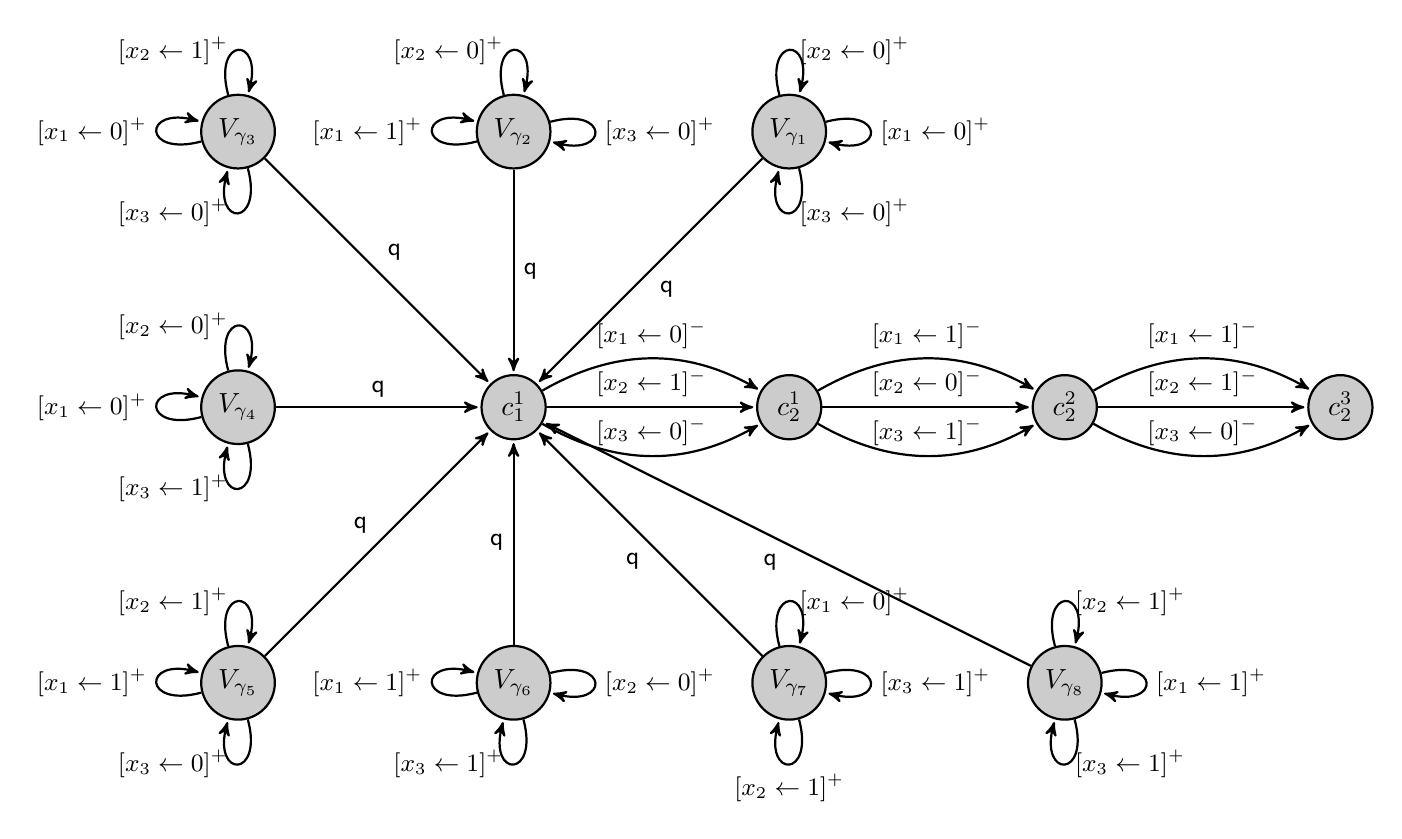
\begin{tikzpicture}[-,>=stealth',shorten >=1pt,auto,node distance=3.5cm,
  thick,main node/.style={circle,fill=black!20,draw}]

  
  \node[main node] (7) [] {$V_{\gamma_3}$};
  \node[main node] (8) [below of=7] {$V_{\gamma_4}$};
  \node[main node] (9) [below of=8] {$V_{\gamma_5}$};


  \node[main node] (1) [right of=8] {$c_1^1$};
  \node[main node] (2) [right of=1] {$c_2^1$};
  \node[main node] (3) [right of=2] {$c_2^2$};
  \node[main node] (4) [right of=3] {$c_2^3$};

  \node[main node] (5) [above of=2] {$V_{\gamma_1}$};
  \node[main node] (6) [above of=1] {$V_{\gamma_2}$};
  \node[main node] (10) [below of=1] {$V_{\gamma_6}$};
  \node[main node] (11) [below of=2] {$V_{\gamma_7}$};
  \node[main node] (12) [below of=3] {$V_{\gamma_8}$};


  \path[-> , every node/.style={font=\sffamily\small}]
    (5) edge [loop right, right] node  {$[x_1 \leftarrow 0]^+$}   (5)    
    (5) edge [loop above, right] node  {$[x_2 \leftarrow 0]^+$}  (5)    
    (5) edge [loop below, right] node  {$[x_3 \leftarrow 0]^+$}  (5)

    (5) edge [] node  {q}  (1)    
    

    (6) edge [loop left, left] node   {$[x_1 \leftarrow 1]^+$}   (6)    
    (6) edge [loop above, left] node  {$[x_2 \leftarrow 0]^+$}  (6)    
    (6) edge [loop right, right] node  {$[x_3 \leftarrow 0]^+$}  (6)

    (6) edge [] node  {q}  (1)    
         


    (7) edge [loop left, left] node   {$[x_1 \leftarrow 0]^+$}   (7)    
    (7) edge [loop above, left] node  {$[x_2 \leftarrow 1]^+$}  (7)    
    (7) edge [loop below, left] node  {$[x_3 \leftarrow 0]^+$}  (7)

    (7) edge [] node   {q}  (1)    
    


    (8) edge [loop left, left] node   {$[x_1 \leftarrow 0]^+$}   (8)    
    (8) edge [loop above, left] node  {$[x_2 \leftarrow 0]^+$}  (8)    
    (8) edge [loop below, left] node  {$[x_3 \leftarrow 1]^+$}  (8)

    (8) edge [] node  {q}  (1)    
    

    (9) edge [loop left, left] node   {$[x_1 \leftarrow 1]^+$}   (9)    
    (9) edge [loop above, left] node  {$[x_2 \leftarrow 1]^+$}  (9)    
    (9) edge [loop below, left] node  {$[x_3 \leftarrow 0]^+$}  (9)

    (9) edge [] node  {q}  (1)    

    
    (10) edge [loop left, left] node   {$[x_1 \leftarrow 1]^+$}   (10)    
    (10) edge [loop right, right] node  {$[x_2 \leftarrow 0]^+$}  (10)    
    (10) edge [loop below, left] node  {$[x_3 \leftarrow 1]^+$}  (10)

    (10) edge [] node   {q}  (1)    

    
    (11) edge [loop above, right] node    {$[x_1 \leftarrow 0]^+$}   (11)    
    (11) edge [loop below, below] node  {$[x_2 \leftarrow 1]^+$}  (11)    
    (11) edge [loop right, right] node  {$[x_3 \leftarrow 1]^+$}  (11)

    (11) edge [] node  {q}  (1)


    (12) edge [loop right, right] node  {$[x_1 \leftarrow 1]^+$}   (12)    
    (12) edge [loop above, right] node  {$[x_2 \leftarrow 1]^+$}  (12)    
    (12) edge [loop below, right] node  {$[x_3 \leftarrow 1]^+$}  (12)

    (12) edge [] node  {q}  (1)    
 

    (1) edge [bend left=30, above] node   {$[x_1 \leftarrow 0]^-$}  (2)
    (1) edge [bend left=0, above] node   {$[x_2 \leftarrow 1]^-$}  (2)
    (1) edge [bend right=30, above] node   {$[x_3 \leftarrow 0]^-$}  (2)
      

    (2) edge [bend left=30, above] node  {$[x_1 \leftarrow 1]^-$}  (3)
    (2) edge [bend left=0, above] node  {$[x_2 \leftarrow 0]^-$}  (3)
    (2) edge [bend right=30, above] node  {$[x_3 \leftarrow 1]^-$}  (3)
   

    (3) edge [bend left=30, above] node  {$[x_1 \leftarrow 1]^-$}  (4)
    (3) edge [bend left=0, above] node  {$[x_2 \leftarrow 1]^-$}  (4)
    (3) edge [bend right=30, above] node  {$[x_3 \leftarrow 0]^-$}  (4)
    
    ;

\end{tikzpicture}
\caption{Example of graph for $\Phi$}
\label{fig:sat_to_cfpq_graph_example}
\end{figure*}

\section{Reduction to $k/3$}

	
Firs step is to split variables into three group of the same size.
Suppose this splitting preserves the order.
So, we have a set of partial substitution. 

By the same way we create vertices for partial subctitutions.


\section{An Example of Reduction $k/3$}

For our example:
\begin{align*}
\gamma_1^1 = \{x_1 \leftarrow 1 \} \\
\gamma_1^2 = \{x_1 \leftarrow 0 \} \\
\gamma_2^1 = \{x_2 \leftarrow 1 \} \\
\gamma_2^2 = \{x_2 \leftarrow 0 \} \\
\gamma_3^1 = \{x_3 \leftarrow 1 \} \\
\gamma_3^2 = \{x_3 \leftarrow 0 \} 
\end{align*}

Grammar:
\begin{align*}
S & \to S_1 \mid S_2 \mid S_3 \mid S_4 \mid S_5 \mid S_6 \mid S_7 \mid S_8\\
S_1 & \to q \mid p^+ \ S_1 \ p^- 
      \mid [x_1 \leftarrow 0]^+ \ S_1 \ [x_1 \leftarrow 0]^- \\ 
    & \mid [x_2 \leftarrow 0]^+ \ S_1 \ [x_2 \leftarrow 0]^- 
      \mid [x_3 \leftarrow 0]^+ \ S_1 \ [x_3 \leftarrow 0]^- \\
S_2 & \to q \\
    & \mid p^+ \ S_2 \ p^- 
      \mid [x_1 \leftarrow 1]^+ \ S_2 \ [x_1 \leftarrow 1]^- \\ 
    & \mid [x_2 \leftarrow 0]^+ \ S_2 \ [x_2 \leftarrow 0]^- 
      \mid [x_3 \leftarrow 0]^+ \ S_2 \ [x_3 \leftarrow 0]^- \\
S_3 & \to q \mid p^+ \ S_3 \ p^- 
      \mid [x_1 \leftarrow 0]^+ \ S_3 \ [x_1 \leftarrow 0]^- \\ 
    & \mid [x_2 \leftarrow 1]^+ \ S_3 \ [x_2 \leftarrow 1]^- 
      \mid [x_3 \leftarrow 0]^+ \ S_3 \ [x_3 \leftarrow 0]^- \\
S_4 & \to q \mid p^+ \ S_4 \ p^- 
      \mid [x_1 \leftarrow 0]^+ \ S_4 \ [x_1 \leftarrow 0]^- \\ 
    & \mid [x_2 \leftarrow 0]^+ \ S_4 \ [x_2 \leftarrow 0]^- 
      \mid [x_3 \leftarrow 1]^+ \ S_4 \ [x_3 \leftarrow 1]^- \\
S_5 & \to q \mid p^+ \ S_5 \ p^- 
      \mid [x_1 \leftarrow 1]^+ \ S_5 \ [x_1 \leftarrow 1]^- \\ 
    & \mid [x_2 \leftarrow 1]^+ \ S_5 \ [x_2 \leftarrow 1]^- 
      \mid [x_3 \leftarrow 0]^+ \ S_5 \ [x_3 \leftarrow 0]^- \\
S_6 & \to q \mid p^+ \ S_6 \ p^- 
      \mid [x_1 \leftarrow 1]^+ \ S_6 \ [x_1 \leftarrow 1]^- \\ 
    & \mid [x_2 \leftarrow 0]^+ \ S_6 \ [x_2 \leftarrow 0]^- 
      \mid [x_3 \leftarrow 1]^+ \ S_6 \ [x_3 \leftarrow 1]^- \\
S_3 & \to q \mid p^+ \ S_7 \ p^- 
      \mid [x_1 \leftarrow 0]^+ \ S_7 \ [x_1 \leftarrow 0]^- \\ 
    & \mid [x_2 \leftarrow 1]^+ \ S_7 \ [x_2 \leftarrow 1]^- 
      \mid [x_3 \leftarrow 1]^+ \ S_7 \ [x_3 \leftarrow 1]^- \\
S_8 & \to q \mid p^+ \ S_8 \ p^- 
      \mid [x_1 \leftarrow 1]^+ \ S_8 \ [x_1 \leftarrow 1]^- \\ 
    & \mid [x_2 \leftarrow 1]^+ \ S_8 \ [x_2 \leftarrow 1]^- 
      \mid [x_3 \leftarrow 1]^+ \ S_8 \ [x_3 \leftarrow 1]^- \\
\end{align*}

\begin{figure*}
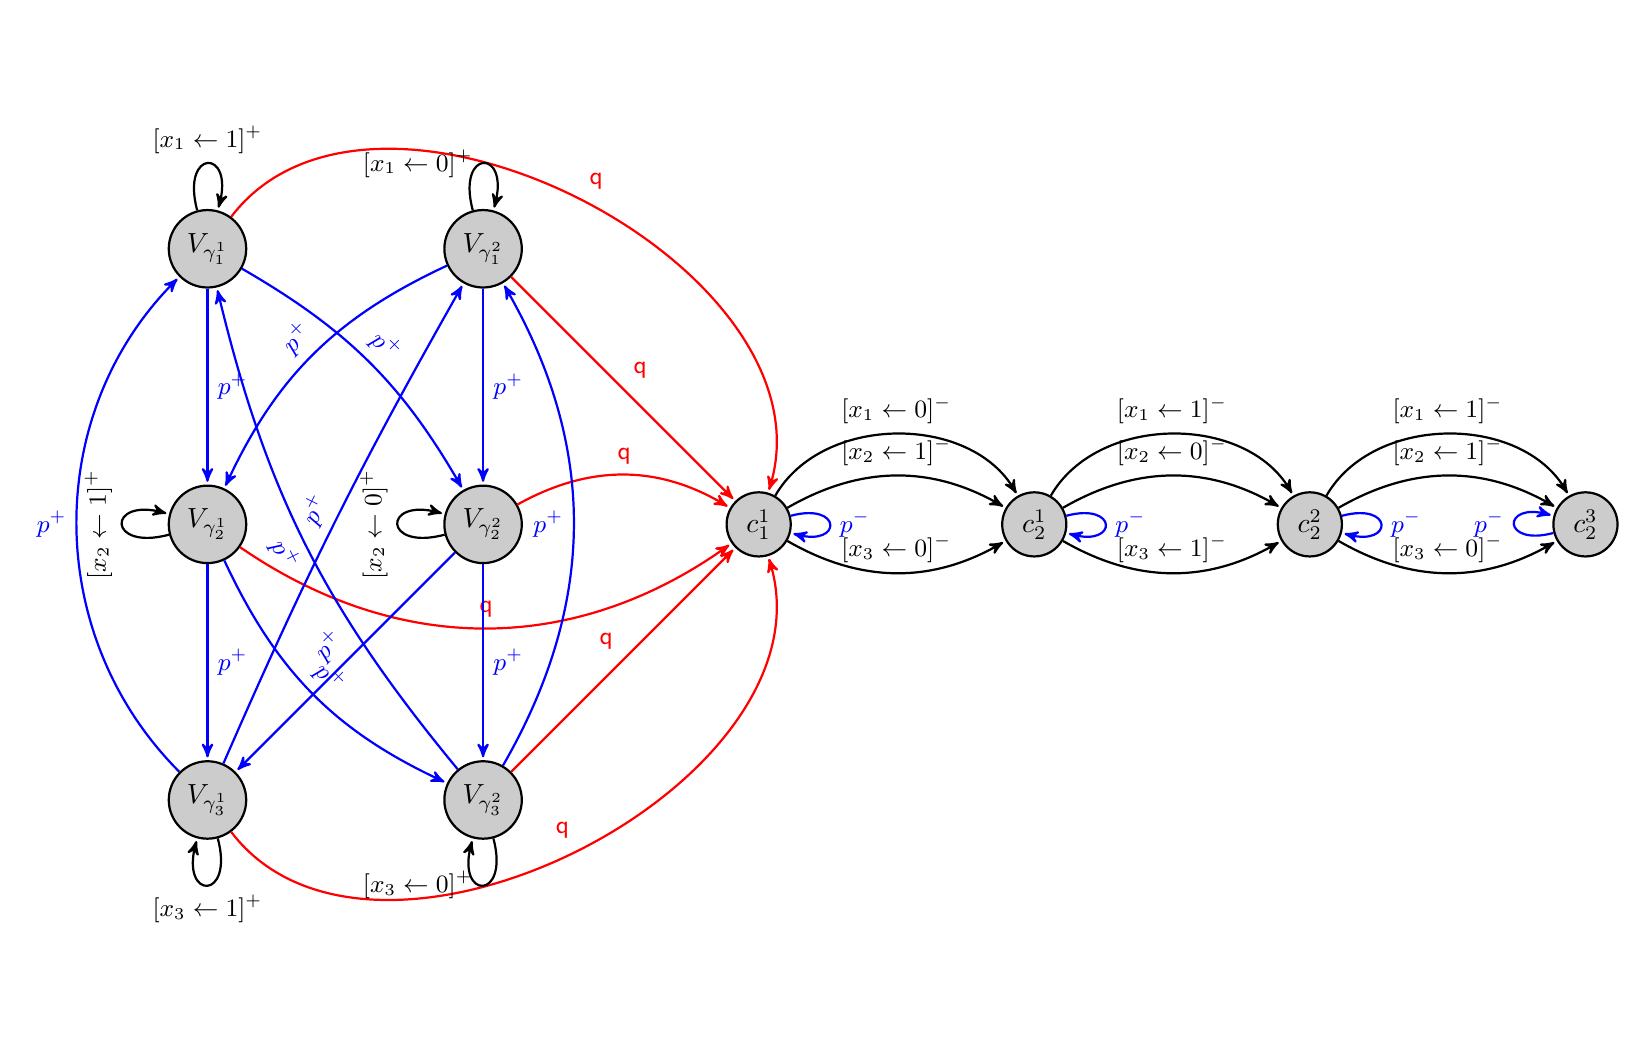
\begin{tikzpicture}[-,>=stealth',shorten >=1pt,auto,node distance=3.5cm,
  thick,main node/.style={circle,fill=black!20,draw}]

  
  \node[main node] (6) [] {$V_{\gamma_1^1}$};
  \node[main node] (7) [right of =6] {$V_{\gamma_1^2}$};
  \node[main node] (8) [below of=6] {$V_{\gamma_2^1}$};
  \node[main node] (9) [right of=8] {$V_{\gamma_2^2}$};
  \node[main node] (10) [below of=8] {$V_{\gamma_3^1}$};
  \node[main node] (11) [right of=10] {$V_{\gamma_3^2}$};
  


  \node[main node] (1) [right of=9] {$c_1^1$};
  \node[main node] (2) [right of=1] {$c_2^1$};
  \node[main node] (3) [right of=2] {$c_2^2$};
  \node[main node] (4) [right of=3] {$c_2^3$};

  
  \path[-> , every node/.style={font=\sffamily\small}]
    (6) edge [loop above, above] node  {$[x_1 \leftarrow 1]^+$}   (6)    
    
    (6) edge [bend left = 80, color=red] node  {q}  (1)        
    (6) edge [color=blue] node  {$p^+$}  (8)
    (6) edge [color=blue, sloped, bend left=15] node  {$p^+$}  (9)                


    (7) edge [loop above, left] node  {$[x_1 \leftarrow 0]^+$}   (7)    
    
    (7) edge [color=red] node {q}  (1)        
    (7) edge [color=blue, sloped, above, bend right=20] node  {$p^+$}  (8)
    (7) edge [color=blue] node  {$p^+$}  (9) 


    (8) edge [loop left, sloped, above] node  {$[x_2 \leftarrow 1]^+$}   (8)    
    
    (8) edge [bend right=35, sloped, above, color=red] node  {q}  (1)        
    (8) edge [color=blue] node  {$p^+$}  (10)
    (8) edge [color=blue, sloped, bend right=20] node  {$p^+$}  (11) 

    (9) edge [loop left, above, sloped] node  {$[x_2 \leftarrow 0]^+$}   (9)    
    
    (9) edge [color=red,bend left] node  {q}  (1)        
    (9) edge [color=blue, sloped, above] node  {$p^+$}  (10)
    (9) edge [color=blue] node  {$p^+$}  (11)     
    
    (10) edge [loop below, below] node  {$[x_3 \leftarrow 1]^+$}   (10)    
    
    (10) edge [bend right=80,color=red] node  {q}  (1)        
    (10) edge [bend left=45, color=blue] node  {$p^+$}  (6)
    (10) edge [bend left=3, color=blue, above, sloped] node  {$p^+$}  (7) 
    
    (11) edge [loop below, left] node  {$[x_3 \leftarrow 0]^+$}   (11)    
    
    (11) edge [color=red] node  {q}  (1) 
    (11) edge [bend left=13, color=blue, below, sloped] node  {$p^+$}  (6)
    (11) edge [bend right, color=blue] node  {$p^+$}  (7)


    (1) edge [bend left=60, above] node  {$[x_1 \leftarrow 0]^-$}  (2)
    (1) edge [bend left=30, above] node  {$[x_2 \leftarrow 1]^-$}  (2)
    (1) edge [bend right=30, above] node  {$[x_3 \leftarrow 0]^-$}  (2)
    (1) edge [loop right, right, color=blue] node {$p^-$} (1)
    


    (2) edge [bend left=60, above] node  {$[x_1 \leftarrow 1]^-$}  (3)
    (2) edge [bend left=30, above] node  {$[x_2 \leftarrow 0]^-$}  (3)
    (2) edge [bend right=30, above] node  {$[x_3 \leftarrow 1]^-$}  (3)
    (2) edge [loop right, right, color=blue] node {$p^-$} (2)
    

    (3) edge [bend left=60, above] node  {$[x_1 \leftarrow 1]^-$}  (4)
    (3) edge [bend left=30, above] node  {$[x_2 \leftarrow 1]^-$}  (4)
    (3) edge [bend right=30, above] node  {$[x_3 \leftarrow 0]^-$}  (4)
    (3) edge [loop right, right, color=blue] node {$p^-$} (3)
    
    (4) edge [loop left, left, color=blue] node {$p^-$} (4)
    

    ;

\end{tikzpicture}
\caption{Example of graph for $\Phi$}
\label{fig:sat_to_cfpq_graph_example}
\end{figure*}


\section{Improved Reduction to $k/3$}

	
Firs step is to split variables into three group of the same size.
Suppose this splitting preserves the order.
So, we have a set of partial substitution. 

By the same way we create vertices for partial subctitutions.


\section{An Example of Improved Reduction $k/3$}

For our example:
\begin{align*}
\gamma_1^1 = \{x_1 \leftarrow 1 \} \\
\gamma_1^2 = \{x_1 \leftarrow 0 \} \\
\gamma_2^1 = \{x_2 \leftarrow 1 \} \\
\gamma_2^2 = \{x_2 \leftarrow 0 \} \\
\gamma_3^1 = \{x_3 \leftarrow 1 \} \\
\gamma_3^2 = \{x_3 \leftarrow 0 \} 
\end{align*}

Grammar:
\begin{align*}
S & \to S_{\gamma_1} \mid S_{\gamma_2} \mid S_{\gamma_3} \mid S_{\gamma_4} \mid S_{\gamma_5} \mid S_{\gamma_6} \mid S_{\gamma_7} \mid S_{\gamma_8}\\
S_1 & \to q  
      \mid [x_1 \leftarrow 1]^+ \ S_1 \ [x_1 \leftarrow 1]^- \\ 
S_2 & \to q  
      \mid [x_1 \leftarrow 0]^+ \ S_2 \ [x_1 \leftarrow 0]^- \\ 
S_3 & \to q  
      \mid [x_2 \leftarrow 1]^+ \ S_3 \ [x_2 \leftarrow 1]^- \\ 
S_4 & \to q 
      \mid [x_2 \leftarrow 0]^+ \ S_4 \ [x_2 \leftarrow 0]^- \\ 
S_5 & \to q
      \mid [x_3 \leftarrow 1]^+ \ S_5 \ [x_3 \leftarrow 1]^- \\ 
S_6 & \to q
      \mid [x_3 \leftarrow 0]^+ \ S_6 \ [x_3 \leftarrow 0]^- \\ 
S_{\gamma_1} & \to S_2 \mid S_4 \mid S_6 \mid S_{\gamma_1} \ p \ S_2 \mid S_{\gamma_1} \ p \ S_4 \mid S_{\gamma_1} \ p \ S_6\\
S_{\gamma_2} & \to S_1 \mid S_4 \mid S_6 \mid S_{\gamma_2} \ p \ S_1 \mid S_{\gamma_2} \ p \ S_4 \mid S_{\gamma_2} \ p \ S_6\\
S_{\gamma_3} & \to S_2 \mid S_3 \mid S_6 \mid S_{\gamma_3} \ p \ S_2 \mid S_{\gamma_3} \ p \ S_3 \mid S_{\gamma_3} \ p \ S_6\\
S_{\gamma_4} & \to S_2 \mid S_4 \mid S_5 \mid S_{\gamma_4} \ p \ S_2 \mid S_{\gamma_4} \ p \ S_4 \mid S_{\gamma_4} \ p \ S_5\\
S_{\gamma_5} & \to S_1 \mid S_3 \mid S_6 \mid S_{\gamma_5} \ p \ S_1 \mid S_{\gamma_5} \ p \ S_3 \mid S_{\gamma_5} \ p \ S_6\\
S_{\gamma_6} & \to S_1 \mid S_4 \mid S_5 \mid S_{\gamma_6} \ p \ S_1 \mid S_{\gamma_6} \ p \ S_4 \mid S_{\gamma_6} \ p \ S_5\\
S_{\gamma_7} & \to S_2 \mid S_3 \mid S_5 \mid S_{\gamma_7} \ p \ S_2 \mid S_{\gamma_7} \ p \ S_3 \mid S_{\gamma_7} \ p \ S_5\\
S_{\gamma_8} & \to S_1 \mid S_3 \mid S_5 \mid S_{\gamma_8} \ p \ S_1 \mid S_{\gamma_8} \ p \ S_3 \mid S_{\gamma_8} \ p \ S_5\\
\end{align*}


Grammar in EBNF (better for tensor-based algorithm):
\begin{align*}
S & \to S_{\gamma_1} \mid S_{\gamma_2} \mid S_{\gamma_3} \mid S_{\gamma_4} \mid S_{\gamma_5} \mid S_{\gamma_6} \mid S_{\gamma_7} \mid S_{\gamma_8}\\
S_1 & \to q  
      \mid [x_1 \leftarrow 1]^+ \ S_1 \ [x_1 \leftarrow 1]^- \\ 
S_2 & \to q  
      \mid [x_1 \leftarrow 0]^+ \ S_2 \ [x_1 \leftarrow 0]^- \\ 
S_3 & \to q  
      \mid [x_2 \leftarrow 1]^+ \ S_3 \ [x_2 \leftarrow 1]^- \\ 
S_4 & \to q 
      \mid [x_2 \leftarrow 0]^+ \ S_4 \ [x_2 \leftarrow 0]^- \\ 
S_5 & \to q
      \mid [x_3 \leftarrow 1]^+ \ S_5 \ [x_3 \leftarrow 1]^- \\ 
S_6 & \to q
      \mid [x_3 \leftarrow 0]^+ \ S_6 \ [x_3 \leftarrow 0]^- \\ 
S_{\gamma_1} & \to (S_2 \mid S_4 \mid S_6) (p \ (S_2 \mid S_4 \mid S_6))^*\\
S_{\gamma_2} & \to (S_1 \mid S_4 \mid S_6) (p \ (S_1 \mid S_4 \mid S_6))^*\\
S_{\gamma_3} & \to (S_2 \mid S_3 \mid S_6) (p \ (S_2 \mid S_3 \mid S_6))^*\\
S_{\gamma_4} & \to (S_2 \mid S_4 \mid S_5) (p \ (S_2 \mid S_4 \mid S_5))^*\\
S_{\gamma_5} & \to (S_1 \mid S_3 \mid S_6) (p \ (S_1 \mid S_3 \mid S_6))^*\\
S_{\gamma_6} & \to (S_1 \mid S_4 \mid S_5) (p \ (S_1 \mid S_4 \mid S_5))^*\\
S_{\gamma_7} & \to (S_2 \mid S_3 \mid S_5) (p \ (S_2 \mid S_3 \mid S_5))^*\\
S_{\gamma_8} & \to (S_1 \mid S_3 \mid S_5) (p \ (S_1 \mid S_3 \mid S_5))^*\\
\end{align*}


\begin{figure*}
\begin{tikzpicture}[-,>=stealth',shorten >=1pt,auto,node distance=3.5cm,
  thick,main node/.style={circle,fill=black!20,draw}]

  \node[main node] (1) [right of=9] {$c_1^1$};
  \node[main node] (2) [right of=1] {$c_2^1$};
  \node[main node] (3) [right of=2] {$c_2^2$};
  \node[main node] (4) [right of=3] {$c_2^3$};


  \node[main node] (6) [above of=3] {$V_{\gamma_1^1}$};
  \node[main node] (7) [above of=2] {$V_{\gamma_1^2}$};
  \node[main node] (8) [above of=1] {$V_{\gamma_2^1}$};
  \node[main node] (9) [below of=1] {$V_{\gamma_2^2}$};
  \node[main node] (10) [below of=2] {$V_{\gamma_3^1}$};
  \node[main node] (11) [below of=3] {$V_{\gamma_3^2}$};
  

  
  \path[-> , every node/.style={font=\sffamily\small}]
    (6) edge [loop above, above] node  {$[x_1 \leftarrow 1]^+$}   (6)    
    (6) edge [bend left=5, color=red] node  {q}  (1)        
    (6) edge [bend left=5, color=red] node  {q}  (2)        
    (6) edge [bend left=5, color=red] node  {q}  (3)        
    (1) edge [bend left=5, color=blue] node  {p}  (6)        
    (2) edge [bend left=5, color=blue] node  {p}  (6)        
    (3) edge [bend left=5, color=blue] node  {p}  (6)    

    (7) edge [loop above, above] node  {$[x_1 \leftarrow 0]^+$}   (7)    
    (7) edge [bend left=5, color=red] node  {q}  (1)        
    (7) edge [bend left=5, color=red] node  {q}  (2)        
    (7) edge [bend left=5, color=red] node  {q}  (3)        
    (1) edge [bend left=5, color=blue] node  {p}  (7)        
    (2) edge [bend left=5, color=blue] node  {p}  (7)        
    (3) edge [bend left=5, color=blue] node  {p}  (7)    

    (8) edge [loop above, above] node  {$[x_2 \leftarrow 1]^+$}   (8)    
    (8) edge [bend left=5, color=red] node  {q}  (1)        
    (8) edge [bend left=5, color=red] node  {q}  (2)        
    (8) edge [bend left=5, color=red] node  {q}  (3)        
    (1) edge [bend left=5, color=blue] node  {p}  (8)        
    (2) edge [bend left=5, color=blue] node  {p}  (8)        
    (3) edge [bend left=5, color=blue] node  {p}  (8)    

    (9) edge [loop below, below] node  {$[x_2 \leftarrow 0]^+$}   (9)    
    (9) edge [bend left=5, color=red] node  {q}  (1)        
    (9) edge [bend left=5, color=red] node  {q}  (2)        
    (9) edge [bend left=5, color=red] node  {q}  (3)        
    (1) edge [bend left=5, color=blue] node  {p}  (9)        
    (2) edge [bend left=5, color=blue] node  {p}  (9)        
    (3) edge [bend left=5, color=blue] node  {p}  (9)    
    
    (10) edge [loop below, below] node  {$[x_3 \leftarrow 1]^+$}   (10)    
    (10) edge [bend left=5, color=red] node  {q}  (1)        
    (10) edge [bend left=5, color=red] node  {q}  (2)        
    (10) edge [bend left=5, color=red] node  {q}  (3)        
    (1) edge [bend left=5, color=blue] node  {p}  (10)        
    (2) edge [bend left=5, color=blue] node  {p}  (10)        
    (3) edge [bend left=5, color=blue] node  {p}  (10)    
    
    (11) edge [loop below, below] node  {$[x_3 \leftarrow 0]^+$}   (11)    
    (11) edge [bend left=5, color=red] node  {q}  (1)        
    (11) edge [bend left=5, color=red] node  {q}  (2)        
    (11) edge [bend left=5, color=red] node  {q}  (3)        
    (1) edge [bend left=5, color=blue] node  {p}  (11)        
    (2) edge [bend left=5, color=blue] node  {p}  (11)        
    (3) edge [bend left=5, color=blue] node  {p}  (11)    
    

    (1) edge [bend left=30, above] node  {$[x_1 \leftarrow 0]^-$}  (2)
    (1) edge [bend left=0, above] node  {$[x_2 \leftarrow 1]^-$}  (2)
    (1) edge [bend right=30, above] node  {$[x_3 \leftarrow 0]^-$}  (2)
    
    (2) edge [bend left=30, above] node  {$[x_1 \leftarrow 1]^-$}  (3)
    (2) edge [bend left=0, above] node  {$[x_2 \leftarrow 0]^-$}  (3)
    (2) edge [bend right=30, above] node  {$[x_3 \leftarrow 1]^-$}  (3)
    
    (3) edge [bend left=30, above] node  {$[x_1 \leftarrow 1]^-$}  (4)
    (3) edge [bend left=0, above] node  {$[x_2 \leftarrow 1]^-$}  (4)
    (3) edge [bend right=30, above] node  {$[x_3 \leftarrow 0]^-$}  (4)

    ;

\end{tikzpicture}
\caption{Example of graph for $\Phi$}
\label{fig:sat_to_cfpq_graph_example}
\end{figure*}
\section{From Arbitrary CFPQ to Dyck Query}\label{sec:cfpq_to_dyck}

This reduction is inspired by the construction described in~\cite{OptimalDLR}.

Consider a context-free grammar $\mathcal{G}=(\Sigma, N, P, S)$ in BNF where $\Sigma$ is a terminal alphabet, $N$ is 
a nonterminal alphabet, $P$ is a set of productions, $S \in N$ is a start nonterminal.
Also we denote a directed labeled graph by $G=(V,E,L)$ where $E \subseteq V \times L \times V$ and $L \subseteq \Sigma$. 

We should construct new input graph $G'$ and new grammar $\mathcal{G'}$ such that $\mathcal{G'}$ specifies a Dyck language and there is a simple mapping from $\text{CFPQ}(\mathcal{G'}, G')$ to $\text{CFPQ}(\mathcal{G}, G)$.
Step-by-step example with description is provided below.
 
Let the input grammar is 
\begin{align*}
S & \rightarrow a \ S \ b \ | \ a \ C \ b 
\\
C & \rightarrow c \ | \ C \ c
\end{align*}

The input graph is presented in fig.~\ref{input}.

\begin{figure}
\resizebox{.5\textwidth}{!}
{
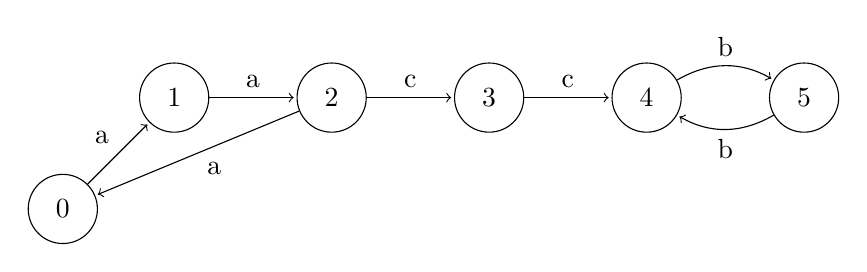
\begin{tikzpicture}[shorten >=1pt,node distance=2cm,on grid,auto] 
   \node[state] (q_0)   {$0$}; 
   \node[state] (q_1) [above right=of q_0] {$1$}; 
   \node[state] (q_2) [right=of q_1] {$2$}; 
   \node[state] (q_3) [right=of q_2] {$3$};
   \node[state] (q_4) [right=of q_3] {$4$};
   \node[state] (q_5) [right=of q_4] {$5$};
    \path[->] 
    (q_0) edge  node {a} (q_1)          
    (q_1) edge  node {a} (q_2)
    (q_2) edge  node {a} (q_0)
    (q_2) edge  node {c} (q_3)
    (q_3) edge  node {c} (q_4)
    (q_4) edge[bend left, above]  node {b} (q_5)
    (q_5) edge[bend left, below]  node {b} (q_4);
\end{tikzpicture}
}

\caption{The input graph}
\label{input}
\end{figure}

\begin{enumerate}
\item Let $\Sigma_{()} =\{ t_( , t_)  | t \in \Sigma \}$.
\item Let $N_{()} = \{ N_( , N_) | N \in N  \}$.
\item Let $M_{\mathcal{G}} = (V_{\mathcal{G}}, E_{\mathcal{G}}, L_{\mathcal{G}})$ is a directed 
labeled graph, where $L_{\mathcal{G}} \subseteq (\Sigma_{()} \cup N_{()})$.
This graph is created the same manner as described in~\cite{OptimalDLR} but we do not require the grammar be in CNF.
Let $x \in V_{\mathcal{G}}$ and $y \in V_{\mathcal{G}}$ is ``start'' and ``final'' vertices respectively. 
This graph may be treated as a finite automaton, so it can be minimized and we can compute an $\varepsilon$-closure if the input grammar contains $\varepsilon$ productions.
The graph $M_{\mathcal{G}}$ for our example is presented in fig.~\ref{mod}.

\begin{figure}
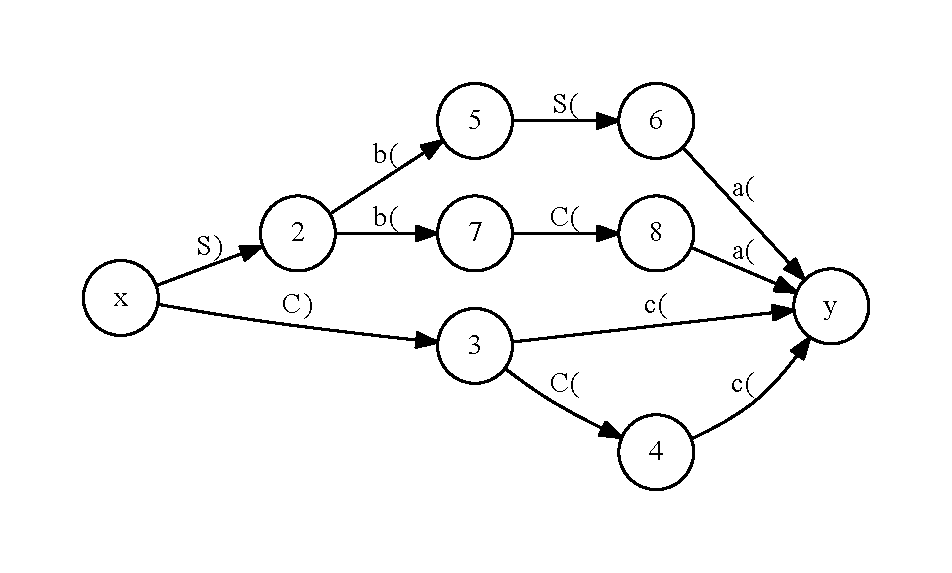
\includegraphics[width=.5\textwidth]{dot/grammar_1.pdf}

\caption{The $M_{\mathcal{G}}$ graph}
\label{mod}

\end{figure}


The minimized graph is presented in fig.~\ref{minimized}.
\begin{figure}
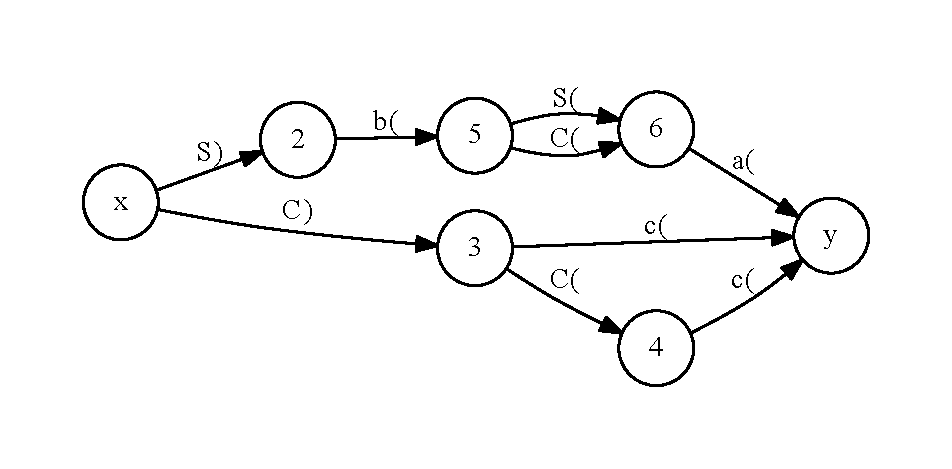
\includegraphics[width=.5\textwidth]{dot/grammar_min.pdf}


\caption{The minimized $M_{\mathcal{G}}$}
\label{minimized}

\end{figure}


\item For each $v \in V$ create $M_{\mathcal{G}}^v$: unique instance of $M_{\mathcal{G}}$.
\item New graph $G^{'}$ is a graph $G$ where each label $t$ is replaced with $t_{)}^i$ and some additional edges are created:
\begin{itemize}
\item Add an edge $(v', S_(, v)$ for each $v \in V$. 
\item And the respective $M_{\mathcal{G}}^v$ for each $v \in V$:
  \begin{itemize}
    \item reattach all edges outgoing from $x^v$ (``start'' vertex of $M_{\mathcal{G}}^v$) to $v$;
    \item reattach all edges incoming to $y^v$ (``final'' vertex of $M_{\mathcal{G}}^v$) to $v$.    
  \end{itemize}
  New input graph is ready. It is presented in fig.~\ref{newInput}.

\begin{figure*}  
  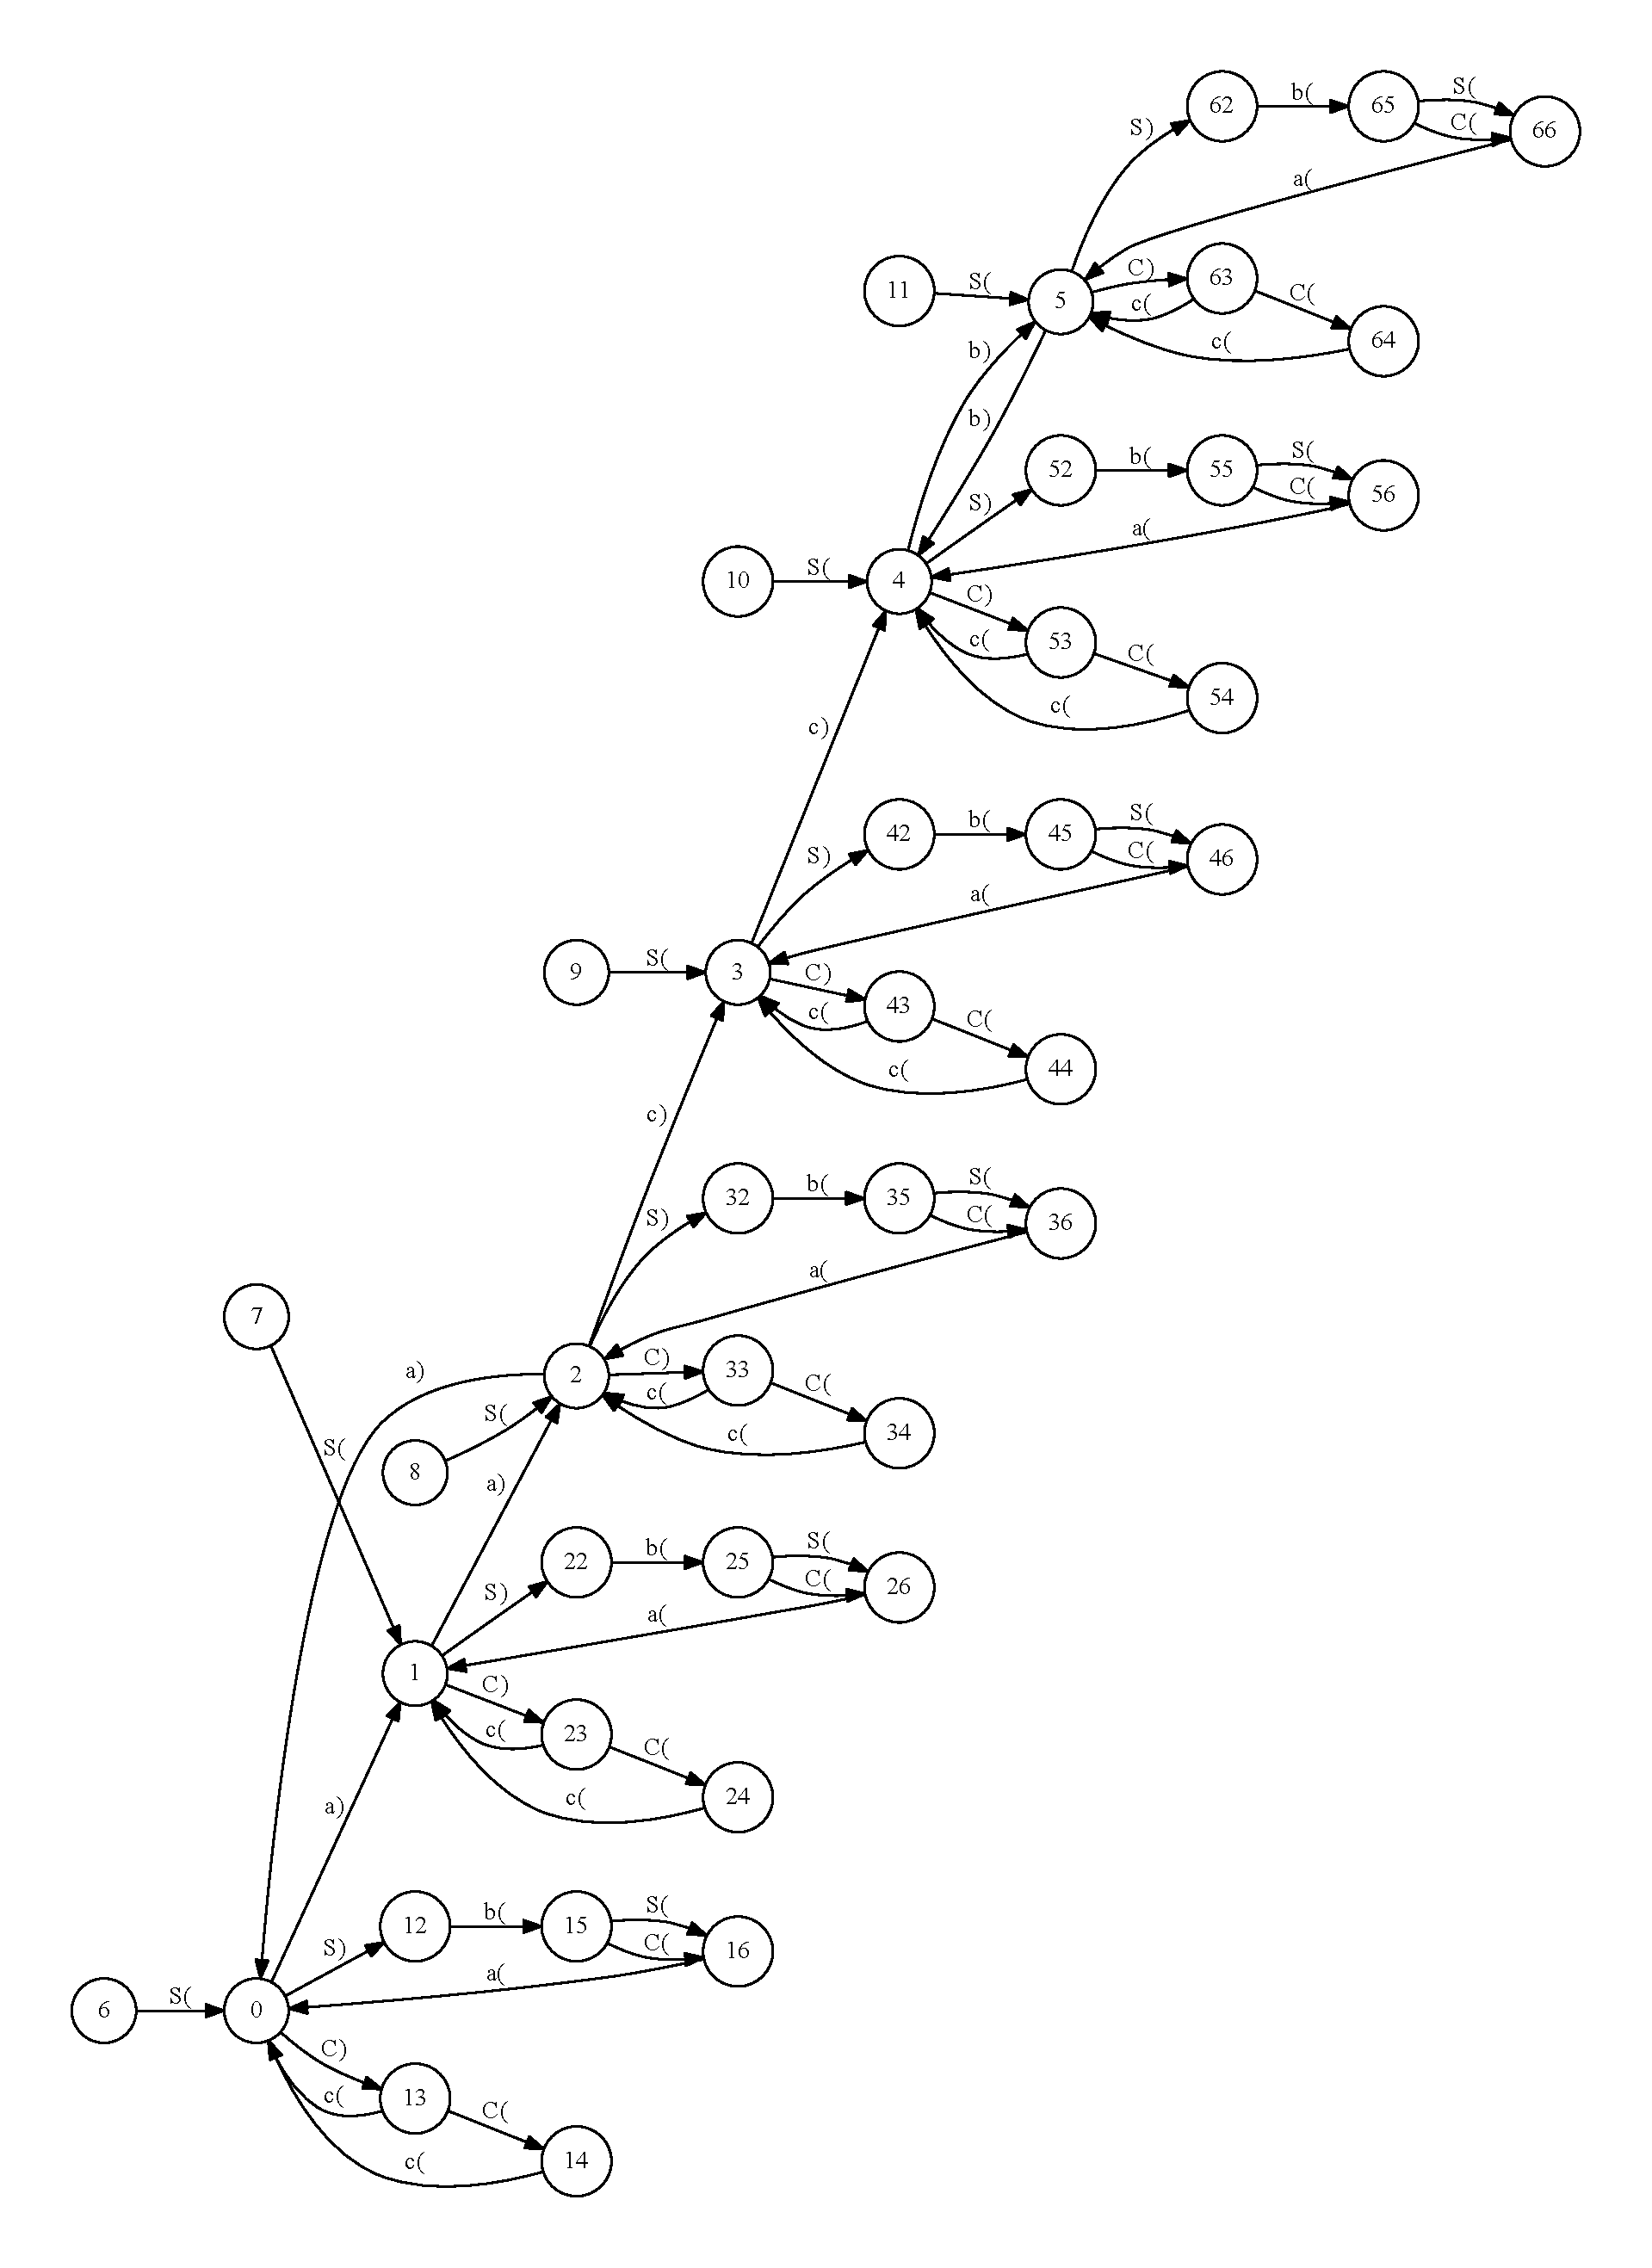
\includegraphics[width=.9\textwidth]{dot/input_new_min.pdf}
 
  \caption{New input graph}
  \label{newInput}

\end{figure*}

\end{itemize}

\item New grammar $\mathcal{G'}=(\Sigma^{'}, N', P', S')$ where $\Sigma^{'} = \Sigma_{()} \cup N_{()}$, $N' = \{ S' \}$, $P' = \{ S' \rightarrow b_( \ S' \ b_); S' \rightarrow b_( \ b_) \ | \ b_(, b_{)} \in \Sigma^{'} \} \cup \{ S' \rightarrow S' \ S' \}$ is a set of productions, $S' \in N'$ is a start nonterminal.
\end{enumerate}

Now, if $\text{CFPQ}(\mathcal{G'}, G')$ contains a pair $(u'_0, v')$ such that $e=(u'_0, S_( , u'_1) \in E'$ is an extension edge (step 5, first subitem), then  $(u'_1, v') \in \text{CFPQ}(\mathcal{G}, G)$.
In our example, we can find the following path: $7 \xrightarrow{S_(} 1 \xrightarrow{S_)} 22 \xrightarrow{b_(} 25 \xrightarrow{C_(} 26 \xrightarrow{a_(} 1   
\xrightarrow{a_)} 2 \xrightarrow{C_)} 33 \xrightarrow{C_(} 34 \xrightarrow{c_(} 2  \xrightarrow{c_)} 3 \xrightarrow{C_)} 43 \xrightarrow{c_(} 3 \xrightarrow{c_)} 4 \xrightarrow{b_)} 5$. 
Edge $7 \xrightarrow{S_(} 1$ is the extension, so (1,5) should be in $\text{CFPQ}(\mathcal{G}, G)$ and it is true.



%\input{two_brs}


%\bibliographystyle{abbrv}
\bibliographystyle{ACM-Reference-Format}
\bibliography{SAT_to_CFPQ}



\end{document}